%% Appendix A: detection and line fitting in individual DESI DR1 spectra near P1 and P3
%% (Figure fig:desi_fibers, Table tab:desi_regions)
%% AASTeX sets the appendix in one-column grid: the figure and the (unstarred) table are placed inside the text,
%% because wide floats left pending at the end of the file stall the build before the bibliography.

\section{Detection and line fitting in individual DESI spectra near P1 and P3}\label{sec:appendix-desi}

This appendix describes the DESI measurements within $0.5^\circ$ of the W26 regions P1 $(\alpha,\delta)=(116\fdg65,+16\fdg60)$ and P3 $(116\fdg45,+14\fdg72)$ (Figure~\ref{fig:desi_fibers}; Table~\ref{tab:desi_regions}).

\subsection{Spectra}

The inputs are not DESI sky-fiber spectra: they are public DR1 coadded spectra \citep{DESI2026} of galaxy and quasar targets with no redshift warning, in $\pm40$\,\AA{} line windows (0.8\,\AA{} pixels; vacuum, barycentric). Stars are excluded because their model mismatch falls on the nebular lines. From each coadd we subtract the best-fit model of the pipeline redshift fitter \citep{Guy2023}. The residuals are relative to the petal sky model (Section~\ref{sec:data}): positive on the ridge, negative beside it (Figure~\ref{fig:desi_fibers}a,e).

We analyze 330 (P1) and 530 (P3) coadds, 32\% and 99.8\% of those eligible (retrieval near P1 was incomplete). Two overlapping survey-validation tiles, 80644 (bright program; six nights) and 80683 (dark; four other nights), supply 280 of the P1 coadds and all P3 coadds; the other 50 are main-survey coadds.

\begin{figure*}
\centering
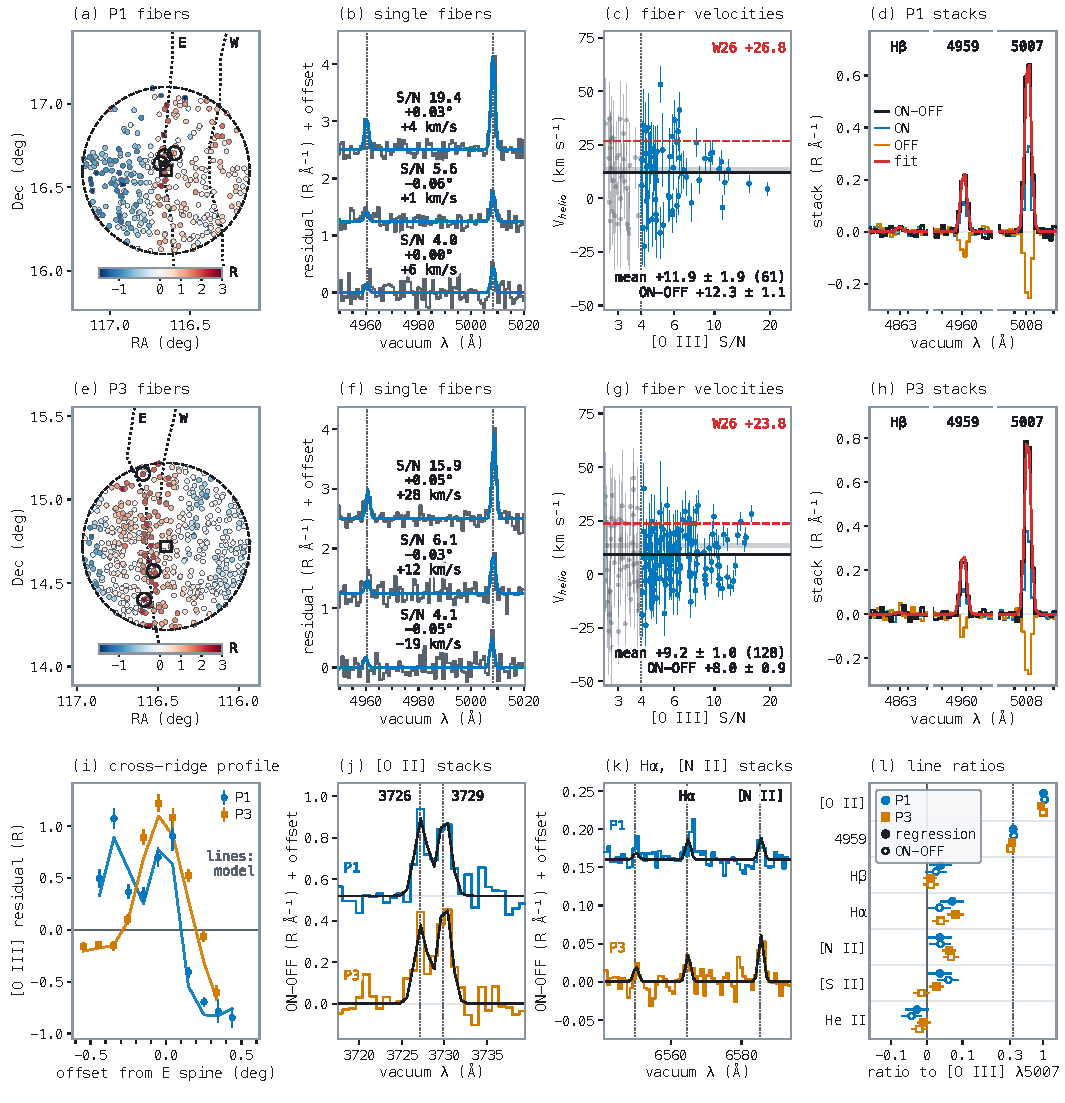
\includegraphics[width=\textwidth]{figures/paper_appendix_desi.pdf}
\caption{DESI DR1 coadds \citep{DESI2026} within $0.5^\circ$ of P1 (top row) and P3 (middle row). (a, e) Fibers with a good fit, colored by petal-relative \Oiii~$\lambda$5007 brightness; dotted lines, E and W strands; dashed circle, $0.5^\circ$ radius; square, region center; rings, the fibers in (b, f). (b, f) Continuum-subtracted residual spectra of the fibers of highest, median and lowest S/N among those with S/N $>4$, with doublet fits; labels give S/N, offset from the E spine and \vhel. (c, g) Fiber \vhel{} against S/N: blue, S/N $>4$; gray, $2.5<$ S/N $\le4$; black line, weighted mean of the blue points; band, adopted value; dashed, W26 Table~4. (d, h) Stacks at \Hb{} and \Oiii~$\lambda\lambda$4959, 5007: ON$-$OFF with fit, ON and OFF. Bottom row, P1 (blue) and P3 (orange): (i) binned residual across the E spine (positive east), with the forward-model prediction (lines); (j, k) ON$-$OFF stacks at \Oii{} and at \Ha{} and \Nii, with fits; (l) ratios to \Oiii~$\lambda$5007 from the regression with intercept (filled) and the ON$-$OFF stack (open); dotted line, 1/2.98.}
\label{fig:desi_fibers}
\end{figure*}

\begin{deluxetable}{lcc}
\tabletypesize{\small}
\tablecaption{DESI DR1 measurements within $0.5^\circ$ of P1 and P3\label{tab:desi_regions}}
\tablehead{\colhead{Quantity} & \colhead{P1} & \colhead{P3}}
\startdata
Coadds: eligible / analyzed / good fit & 1,034 / 330 / 326 & 531 / 530 / 505 \\
Fibers with S/N $>4$ (S/N $<-4$) & 61 (39) & 128 (11) \\
Median per-fiber error (R) & 0.21 & 0.20 \\
Fibers in ON$-$OFF stack: ON, OFF & 161, 175 & 262, 157 \\
\vhel, weighted mean of S/N $>4$ fibers\tablenotemark{a} & $+11.9\pm1.9$ & $+9.2\pm1.0$ \\
\vhel, median of the same fibers & $+13.7\pm2.2$ & $+8.5\pm1.4$ \\
\vhel, ON$-$OFF stack & $+12.3\pm1.1$ & $+8.0\pm0.9$ \\
Model sky brightness at region center (R) & $2.07\pm0.06$ & $1.54\pm0.04$ \\
E-ridge peak (R)\tablenotemark{b} & $1.82\pm0.06$ / $1.83\pm0.06$ / $1.69\pm0.07$ & $1.68\pm0.05$ / $1.65\pm0.03$ / $1.34\pm0.05$ \\
ON$-$OFF mean brightness (R) & $1.36\pm0.05$ & $1.65\pm0.05$ \\
\Oiii~$\lambda5007/\lambda4959$\tablenotemark{c} & 2.91 / 2.97 / 2.87 ($\pm$0.15--0.18) & 3.12 / 3.08 / 3.29 ($\pm$0.17--0.19) \\
\Oii~$\lambda3727$/\Oiii~$\lambda5007$\tablenotemark{c} & 1.00 / 1.03 / 1.05 ($\pm$0.13--0.14) & 0.92 / 0.89 / 0.99 ($\pm$0.09--0.11) \\
\Oii~$\lambda3729/\lambda3726$\tablenotemark{c} & 1.16 / 1.07 / 1.05 ($\pm$0.19--0.24) & 1.28 / 1.26 / 1.32 ($\pm$0.22--0.24) \\
\Oiii~$\lambda5007$/\Hb\tablenotemark{c} & $>9.8$ / $>8.5$ / $>12.0$ & $>21.3$ / $>22.2$ / $>18.1$ \\
\ion{He}{2}~$\lambda4686$/\Oiii~$\lambda5007$ & $<0.08$ & $<0.045$ \\
\Ha/\Oiii~$\lambda5007$ & $<0.16$ & $<0.13$ \\
\Nii~$\lambda6583$/\Oiii~$\lambda5007$ & $<0.13$ & $<0.11$ \\
\Sii~$\lambda\lambda6716,6731$/\Oiii~$\lambda5007$ & $<0.12$ & $<0.06$ \\
\enddata
\tablecomments{Velocities are in \kms{} and exclude the $\pm1.5$\,\kms{} zero-point uncertainty, which these two regions cannot test. Brightnesses use Equation~(\ref{eq:desi_sb}) and exclude the $\approx$20\% acceptance uncertainty of these regions. Ratios are energy ratios; limits are $2\sigma$ and, where one value is given, the weakest of the three estimators. Red-line limits apply to emission that follows the \Oiii{} ridge.}
\tablenotetext{a}{The estimator of Table~\ref{tab:velocity}.}
\tablenotetext{b}{Filament-wide forward model / local fit with the petal term from that model / local fit with a free constant per tile--petal. Uncertainties are bootstraps over fibers.}
\tablenotetext{c}{Regression with intercept / regression with tile--petal means removed / ON$-$OFF stack.}
\end{deluxetable}

\subsection{Line fitting}

For each residual we fit, over 4930--5038\,\AA{} by linear least squares with the pipeline inverse variances, a quadratic continuum plus $A\,[G_{5007}+G_{4959}/2.98]$ (Figure~\ref{fig:desi_fibers}b,f). Here $G$ is a unit-integral Gaussian of fixed dispersion $\sigma=0.759$\,\AA{} (45.5\,\kms) at 5008\,\AA, the quadrature sum of the line-spread function (0.695\,\AA; median of 430 spectra), a 12\,\kms{} intrinsic dispersion and the pixel term. We mask sky lines ($\pm2.5$\,\AA) and the target's own redshifted lines ($\pm8$\,\AA), and clip once at $5\sigma$. The amplitude $A$ at fixed \vhel{} $=+14$\,\kms{} is the $\lambda$5007 flux. The velocity minimizes $\chi^2$ of the same fit on a 2\,\kms{} grid from $-120$ to $+150$\,\kms{} (vacuum rest wavelengths 5008.240 and 4960.295\,\AA); its error follows from the curvature. Other lines are fitted likewise at $+14$\,\kms; the $\lambda5007/\lambda4959$ ratio uses separate fits to the two lines.

Fits pass if at least 60\% of the window is unmasked, the error is below four times the sample median and $|{\rm S/N}|<30$: 326 coadds near P1 and 505 near P3. Of these, 61 and 128 have S/N $>4$ and 39 and 11 have S/N $<-4$; Gaussian noise would give $<0.02$ of each sign. In stacks the line is unresolved (intrinsic FWHM $<40$\,\kms, 97.5\%).

\subsection{Velocities}

The DESI entries of Table~\ref{tab:velocity} are means of the fibers with S/N $>4$ and velocity error $\sigma_V<30$\,\kms, weighted by $1/(\sigma_V^2+5^2)$; the quoted error is the larger of the formal error (1.35 and 0.87\,\kms) and the standard error from the scatter. The fibers scatter more than their formal errors (robust scatter 14.0 and 12.9\,\kms{} against median errors of 10.6 and 9.3\,\kms; Figure~\ref{fig:desi_fibers}c,g), whereas simulated noise gives pulls of rms 1.03--1.05. One cause is that the centroid of a petal-relative residual amplifies velocity differences from the petal mean, here by $\approx$1.9 (P1) and 2.2 (P3).

The petal mean cancels in ON$-$OFF stacks (Figure~\ref{fig:desi_fibers}d,h), formed per tile--petal from fibers with ridge template $T\ge0.5$ (ON) and $T<0.05$ (OFF; anywhere on the petal) and combined with inverse-variance weights; $T$ is the sum of unit-peak Gaussian cross-sections of the traced strands. They give $+12.3\pm1.1$ (P1) and $+8.0\pm0.9$\,\kms{} (P3; bootstrap over fibers), within $1\sigma$ of Table~\ref{tab:velocity}. S/N cuts of 3--8 change the means by $\le1.7$\,\kms, and the two survey-validation tiles differ by $+2.9\pm2.9$ (P1) and $-1.5\pm2.1$\,\kms{} (P3). Within P3, ON$-$OFF gives $+11.2\pm1.1$\,\kms{} east and $+5.5\pm1.0$\,\kms{} west of the E spine (3--4$\sigma$). P1 agrees with the adopted $+13.3\pm1.0$\,\kms; P3 lies 4--5\,\kms{} lower.

\subsection{Line strengths}

DESI fluxes are calibrated for point sources, so a uniform source of surface brightness $I$ yields $F=I\,\Omega/f$, and
\begin{equation}
I=\frac{F f}{\Omega},\qquad I\,[{\rm R}]=0.7428\,f\,F\,[10^{-17}\,{\rm erg\,cm^{-2}\,s^{-1}}]
\label{eq:desi_sb}
\end{equation}
at 5008\,\AA, where $\Omega=\pi(0\farcs76)^2=1.815$\,arcsec$^2$ is the fiber solid angle and $f$ the point-source fiber acceptance (Section~\ref{sec:data}) at the line wavelength.

The predicted residual of fiber $i$ is proportional to $Z_i=T_i-\langle T\rangle$, the mean being over all fiber positions of its tile--petal. The filament-wide forward model (7,345 fibers) and two local fits, with the petal term from that model or a free constant per tile--petal, give E-ridge peaks of 1.69--1.83\,R at P1 and 1.34--1.68\,R at P3 (Figure~\ref{fig:desi_fibers}i), a range that includes the southern-ridge median of 1.62\,R (Section~\ref{sec:brightness}). The spread between models (0.14 and 0.34\,R) exceeds the statistical errors.

DR1 lists no guide-camera acceptance for the two survey-validation tiles; we adopted program medians, $f=0.419$ (bright) and 0.608 (dark). The same ridge then reads $0.94\pm0.06$\,R in tile 80644 against $1.70\pm0.07$\,R in tile 80683 at P1, and $0.99\pm0.07$ against $1.53\pm0.07$\,R at P3, whereas the calibrated fluxes have ratios of $0.80\pm0.06$ and $0.94\pm0.08$ (1.45 expected for the adopted acceptances). Tiles with measured acceptance give $1.62\pm0.16$\,R near P1 (43 fibers). The brightness near P1 and P3 is therefore uncertain by $\approx$20\%, more than the $\pm8\%$ of Section~\ref{sec:data}; the adopted medians enter 46\% of the fibers at Dec $<19.5^\circ$. W26 Table~3 remains 6.2 and 6.6 times the model sky brightness.

\subsection{Line ratios}

We use three estimators: the regression of Section~\ref{sec:data} restricted to each region, with an intercept or with tile--petal means removed, and Gaussian fits to the ON$-$OFF stacks in energy units. Uncertainties are bootstraps over fibers, with floors from the 17 line-free windows (ratio rms 0.029--0.040 at P1 and 0.018--0.022 at P3) and from 300 random OFF$-$OFF splits.

Both regions show an \Oiii{} doublet ratio consistent with 2.98 and \Oii{} at 7--11$\sigma$ (Figure~\ref{fig:desi_fibers}j,l). \Oii/\Oiii{} is within $1\sigma$ of the $1.11$--$1.16$ ($\pm0.08$) measured at Dec $<19.5^\circ$ (Table~\ref{tab:ratios}) at P1 and 1--2$\sigma$ lower at P3. \Hb{} and \ion{He}{2} are undetected; the limits are weaker than the filament-wide ones, except \Oiii/\Hb{} $>18$ at P3.

\Ha{} is positive (0.12--0.19\,R, 5008\,\AA{} equivalent) in both ON and OFF stacks, so the red-line entries limit only emission that follows the \Oiii{} ridge (Figure~\ref{fig:desi_fibers}k). \Nii~$\lambda$6583 at P3 is 0.045--0.068 of \Oiii{} (2.0--3.4$\sigma$; 2.8--4.7$\sigma$ against red null windows alone); the data cannot separate filament \Nii{} from WIM contrast between ridge and off-ridge fibers.

\subsection{Limitations}

The petal sky model was not inspected; its mean is modeled from fiber positions, and near P3 this term ($\approx$0.97\,R) is as large as the signal. Two tiles and at most six tile--petals dominate each region, so the bootstraps over fibers (the regions are too small for the block bootstrap of Section~\ref{sec:data}) do not sample errors shared by a petal.

